% !TEX root = ../main.tex
\section{Regulated pricing-modellen (branche-profit og political support)}\label{thr:regulated-pricing-model}

\paragraph{Definisjon.} BSZ kap.\ 21 presenterer en modell der regulerte priser bestemmes som et kompromiss mellom \emph{brancheprofitt} $\pi(P)$ og \emph{political support} $S(\pi, CS)$. Regulatoren (politikeren) maksimerer ikke velferd direkte, men velger den prisen som maksimerer politisk støtte -- en funksjon av både produsentprofitt og konsumentoverskudd. [SLIDE]

\subsection*{Forklaring}

Modellen bygger på public choice-tradisjonen (Peltzman 1976, Stigler 1971) og forklarer hvorfor regulerte priser typisk er \emph{mellom} monopolpris og marginal\-kostnadspris. [SLIDE/BOK]

\textbf{Byggeklossene:}

\textbf{1. Branche-profit-funksjonen $\pi(P)$.} Bransjens profitt som funksjon av regulert pris $P$:
\begin{itemize}\setlength{\itemsep}{1pt}
\item $\pi(P)$ er null ved $P=AC$ (break-even) og stigende med $P$ opp til monopolpris $P^M$.
\item $\pi(P^M)$ er maksimal profitt; over $P^M$ faller etterspørsel og profitt.
\item Formen er invers-U: $\pi(P)$ stiger fra $P=AC$, topper ved $P^M$, synker deretter.
\end{itemize}

\textbf{2. Konsumentoverskudd $CS(P)$.} Konsumentoverskudd er fallende i $P$: høyere pris $\Rightarrow$ lavere CS.

\textbf{3. Political support-funksjonen $S(\pi, CS)$.} Politikeren vinner støtte fra to grupper:
\begin{itemize}\setlength{\itemsep}{1pt}
\item \textbf{Bransjen/industrien:} lobbyer, kampanjebidrag, arbeidsplasser $\Rightarrow$ støtte stiger i $\pi$.
\item \textbf{Konsumenter/velgere:} stemmer, offentlig opinion $\Rightarrow$ støtte stiger i $CS$.
\item $S$ er stigende i begge, men med avtagende marginaleffekt: $\partial S/\partial \pi > 0$, $\partial S/\partial CS > 0$, $\partial^2 S/\partial \pi^2 < 0$, $\partial^2 S/\partial CS^2 < 0$.
\end{itemize}

\textbf{4. Regulatorens valg.} Regulatoren velger $P^{*}$ som maksimerer $S(\pi(P), CS(P))$:
\[
\frac{dS}{dP} = \frac{\partial S}{\partial \pi}\cdot\pi'(P) + \frac{\partial S}{\partial CS}\cdot CS'(P) = 0
\]
Førsteordensbetingelsen sier at marginal politisk gevinst fra økt brancheprofitt (ved å heve $P$) lik marginal politisk kostnad fra redusert konsumentoverskudd. [BOK]

\textbf{Resultat:} $P^{*}$ ligger mellom $P^{MC}$ (marginal\-kostnadspris, ren konsumentoptimal) og $P^{M}$ (monopolpris, ren bransjeoptimal). Den eksakte plasseringen avhenger av de relative vektene $\partial S/\partial \pi$ vs.\ $\partial S/\partial CS$ -- altså bransjens vs.\ konsumentenes politiske innflytelse.

\subsection*{Grafisk modell -- political support-optimering}

\begin{figure}[h]
\centering
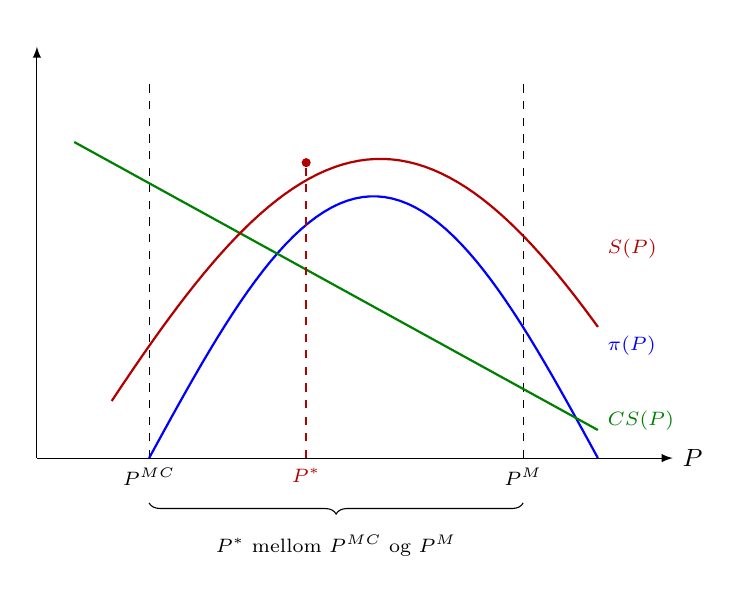
\begin{tikzpicture}[>=latex, scale=0.95, every node/.style={font=\small}]
  % Akser
  \draw[->] (0,0) -- (8.5,0) node[right] {$P$};
  \draw[->] (0,0) -- (0,5.5) node[above] {};
  % MC-pris og monopolpris
  \draw[dashed] (1.5,0) -- (1.5,5.0);
  \node[below] at (1.5,0) {\scriptsize $P^{MC}$};
  \draw[dashed] (6.5,0) -- (6.5,5.0);
  \node[below] at (6.5,0) {\scriptsize $P^{M}$};
  % Profit function pi(P) -- invers U
  \draw[thick, blue, domain=1.5:7.5, samples=60]
    plot (\x, {3.5*sin((\x-1.5)*30)});
  \node[blue, right] at (7.5,1.5) {\scriptsize $\pi(P)$};
  % CS(P) -- fallende
  \draw[thick, green!50!black, domain=0.5:7.5, samples=40]
    plot (\x, {4.5-0.55*\x});
  \node[green!50!black, right] at (7.5,0.5) {\scriptsize $CS(P)$};
  % S(P) -- invers U men toppen forskjøvet til venstre for pi-toppen
  \draw[thick, red!70!black, domain=1.0:7.5, samples=60]
    plot (\x, {4.0*sin((\x-0.5)*22)});
  \node[red!70!black, right] at (7.5,2.8) {\scriptsize $S(P)$};
  % P* optimum
  \draw[thick, dashed, red!70!black] (3.6,0) -- (3.6,4.0);
  \node[below, red!70!black, font=\bfseries] at (3.6,0) {\scriptsize $P^{*}$};
  \filldraw[red!70!black] (3.6,3.95) circle (1.5pt);
  % Brace
  \draw[decorate, decoration={brace, amplitude=4pt, mirror}] (1.5,-0.6) -- (6.5,-0.6);
  \node[below, font=\scriptsize] at (4.0,-0.9) {$P^{*}$ mellom $P^{MC}$ og $P^{M}$};
\end{tikzpicture}
\caption{\textbf{Regulated pricing-modellen.} Brancheprofitt $\pi(P)$ (blå) er invers-U med topp ved monopolpris $P^M$. Konsumentoverskudd $CS(P)$ (grønn) er fallende. Political support $S(P)$ (rød) balanserer de to og topper ved $P^*$ -- mellom $P^{MC}$ og $P^M$. Regulatoren velger $P^*$ der marginal politisk gevinst fra bransjen lik marginal politisk kostnad fra konsumenter. [BOK -- BSZ kap.\ 21]}
\end{figure}

\subsection*{Komparativ statikk}
\begin{itemize}\setlength{\itemsep}{2pt}
\item \textbf{Sterkere bransjelobby} ($\partial S/\partial \pi$ øker): $P^{*}$ skifter mot $P^M$. Eks.: regulerte monopoler med sterk industriorganisasjon.
\item \textbf{Sterkere konsumentpress} ($\partial S/\partial CS$ øker): $P^{*}$ skifter mot $P^{MC}$. Eks.: medieoppmerksomhet, forbrukerorganisasjoner.
\item \textbf{Mer elastisk etterspørsel:} $\pi(P)$ flater ut raskere -- $P^M$ senkes og dermed $P^{*}$.
\end{itemize}

\subsection*{Kjerneforutsetninger}
\begin{itemize}
\item Regulatoren er en rasjonell politisk aktør som maksimerer støtte, ikke velferd.
\item Bransjen og konsumenter konkurrerer om politisk innflytelse via lobbying, stemmer og kampanjebidrag.
\item $S$ er en konkav funksjon av $\pi$ og $CS$ separat (avtagende marginalnytte av begge).
\item Prisen er det eneste reguleringsverktøyet (forenklet).
\end{itemize}

\subsection*{Muligheter}
\begin{itemize}
\item Forklarer hvorfor regulerte priser sjelden er ren MC-prising (for lav profitt gir bransjeprotest) eller ren monopolpris (for lavt CS gir velgerprotest).
\item Predikerer reguleringsutfall som funksjon av relative lobbyingsressurser.
\item Forklarer regulatory capture: når $\partial S/\partial \pi \gg \partial S/\partial CS$, settes $P^{*}\approx P^M$.
\item Forklarer variasjoner i regulering mellom bransjer og land.
\end{itemize}

\subsection*{Begrensninger og kritikk}
\begin{itemize}
\item Reduserer regulering til ren maktkamp -- ignorerer faglige avveininger og juridiske rammer.
\item Forutsetter at regulatoren har full informasjon om $\pi(P)$ og $CS(P)$ -- i praksis strategisk informasjonsasymmetri fra bransjen.
\item Modellen er statisk; reguleringsregimer utvikles over tid med nye aktører, teknologi og politikk.
\item Forutsetter én regulert pris -- i praksis er regulering multidimensjonell (pris, kvalitet, tilgang, investeringskrav).
\item Konsumenter er ofte dårlig organisert (Olsons kollektiv handling-problem) -- modellen undervurderer systematisk bransjens overvekt.
\end{itemize}

\subsection*{Eksempler}
\begin{itemize}\setlength{\itemsep}{2pt}
\item \textbf{Norsk farmasiregulering.} Statens legemiddelverk setter maksimale apotekpriser som balanserer farmasøytisk bransjeprofitt (innovasjonsinsentiv) mot pasientenes betalingsevne. Resultatet: priser lavere enn USA (svakt bransjepress) men høyere enn generiske alternativer (bransjens lobbying mot tvangs-generisk substitusjon). [EKS]
\item \textbf{Norsk taxi-regulering (pre-2020).} Løyvemonopol ga sjåfører monopolprofitt men høye priser. Politisk støtte fra organisertetaxisjåfører (sterk lobby) vs.\ diffuse konsumenter. Deregulering i 2020 skiftet $P^{*}$ nedover etter økt konsumentpress (Uber-debatt). [EKS]
\end{itemize}

\subsection*{Kobling til søyle og andre teorier}
Søyle: \SOne\ (regulatoren allokerer beslutningsrettigheter mellom stat og marked). Relaterte: \thref{market-failure-regulation}{Markedssvikt og regulering}, \thref{externalities}{Eksternaliteter}, \thref{vertical-integration-market-power}{VI og market power}, \thref{principal-agent}{Principal-agent} (regulatoren som agent for velgere).

\paragraph{Brukt i spørsmål:} Q13.
